% !TEX root = saveliev_physics_general_course_2.tex
%!TEX TS-program = pdflatex
%!TEX encoding = UTF-8 Unicode


\chapter[MAXWELL'S EQUATIONS]{MAXWELL'S EQUATIONS}\label{chap:9}
\chaptermark{MAXWELL'S EQUATIONS}

\section{Vortex Electric Field}\label{sec:9_1}

Let us consider electromagnetic induction when a wire loop in which a current is induced is stationary, and the changes in the magnetic flux are due to changes in the magnetic field.
The setting up of an induced current signifies that the changes in the magnetic field produce extraneous forces in the loop that are exerted on the current carriers.
These extraneous forces are associated neither with chemical nor with thermal processes in the wire.
They also cannot be magnetic forces because such forces do not work on charges.
It remains to conclude that the induced current is due to the electric field set up in the wire.
Let us use the symbol $\vec{E}_B$ to denote the strength of this field (this symbol, like the one $\vec{E}_q$ used below, is an auxiliary one; we shall omit the subscripts $B$ and $q$ later on).
The e.m.f. equals the circulation of the vector $\vec{E}_B$ around the given loop:
\begin{equation}\label{eq:9_1}
    \ab{\mathcal{E}}{i} = \oint \vec{E}_B \ccdot \derivec{l}.
\end{equation}

Introducing into \eqn{9_1} $\ab{\mathcal{E}}{i} = -\diffin{\Phi}{t}$ for $\ab{\mathcal{E}}{i}$ and the expression $\int\vec{B}\ccdot\derivec{S}$ for $\Phi$, we arrive at the equation
\begin{equation*}
    \oint \vec{E}_B \ccdot \derivec{l} = -\diff{}{t} \int_S \vec{B} \ccdot \derivec{S}
\end{equation*}

\noindent
(the integral in the right-hand side of the equation is taken over an arbitrary surface resting on the loop).
Since the loop and the surface are stationary, the operations of time differentiation and integration over the surface can have their places exchanged:
\vspace{-12pt}
\begin{equation}\label{eq:9_2}
    \oint \vec{E}_B \ccdot \derivec{l} =  - \int_S \diffpartial{\vec{B}}{t} \ccdot \derivec{S}.
\end{equation}

\noindent
In connection with the fact that the vector $\vec{B}$ depends, generally speaking, both on the time and on the coordinates, we have put the symbol of the partial time derivative inside the integral (the integral $\int\vec{B}\ccdot\derivec{S}$ is a function only of time).

Let us transform the left-hand side of \eqn{9_2} in accordance with Stokes's theorem.
The result is
\begin{equation*}
    \int_S (\curlop{\vec{E}_B}) \ccdot \derivec{S} = - \int_S \diffpartial{\vec{B}}{t} \ccdot \derivec{S}.
\end{equation*}

\noindent
Owing to the arbitrary nature of choosing the integration surface, the following equation must be obeyed:
\begin{equation}\label{eq:9_3}
    \curlop{\vec{E}_B} = - \diffpartial{\vec{B}}{t}.
\end{equation}

\noindent
The curl of the field $\vec{E}_B$ at each point of space equals the time derivative of the vector $\vec{B}$ taken with the opposite sign.

The British physicist James Maxwell (1831-1879) assumed that a time-varying magnetic field causes the field $\vec{E}_B$ to appear in space regardless of whether or not there is a wire loop in this space.
The presence of a loop only makes it possible to detect the existence of an electric field at the corresponding points of space as a result of a current being induced in the loop.

Thus, according to Maxwell's idea, \textit{a time-varying magnetic field gives birth to an electric field}.
This field $\vec{E}_B$ differs appreciably from the electrostatic field $\vec{E}_q$ set up by fixed charges.
An electrostatic field is a potential one, its strength lines begin and terminate at charges.
The curl of the vector $\vec{E}_B$ is zero at any point:
\begin{equation}\label{eq:9_4}
    \curlop{\vec{E}_q} = 0
\end{equation}

\noindent
[see \eqn{1_112}].
According to \eqn{9_3}, the curl of the vector $\vec{E}_B$ differs from zero.
Hence, the field $\vec{E}_B$ like a magnetic field, is a vortex one.
The strength lines of the field $\vec{E}_B$ are closed.

Thus, an electric field may be either a potential ($\vec{E}_q$) or a vortex ($\vec{E}_B$) one.
In the general case, an electric field can consist of the field $\vec{E}_q$ produced by charges and the field $\vec{E}_B$ set up by a time-varying magnetic field.
Adding \eqns{9_3}{9_4}, we get the following equation for the curl of the strength of the total field $\vec{E}=\vec{E}_B+\vec{E}_B$:
\begin{equation}\label{eq:9_5}
    \curlop{\vec{E}} = - \diffpartial{\vec{B}}{t}.
\end{equation}

\noindent
This equation is one of the fundamental ones in Maxwell's electromagnetic theory.

The existence of a relationship between electric and magnetic fields [expressed in particular by \eqn{9_5}] is a reason why the separate treatment of these fields has only a relative meaning.
Indeed, an electric field is set up by a system of fixed charges.
If the charges are fixed relative to a certain inertial reference frame, however, they are moving relative to other inertial frames and, consequently, set up not only an electric, but also a magnetic field.
A stationary wire carrying a steady current sets up a constant magnetic field at every point of space.
This wire is in motion, however, relative to other inertial frames.
Consequently, the magnetic field it sets up at any point with the given coordinates $x$, $y$, $z$ will change and, therefore, give birth to a vortex electric field.
Thus, a field which is ``purely'' electric or ``purely'' magnetic relative to a certain reference frame will be a combination of an electric and a magnetic field forming a single electromagnetic field relative to other reference frames.

\section{Displacement Current}\label{sec:9_2}

For a stationary (\ie, not varying with time) electromagnetic field, the curl of the vector $\vec{H}$ by \eqn{7_9} equals the density of the conduction current at each point:
\begin{equation*}
    \curlop{\vec{H}} = \vec{j}.
\end{equation*}

\noindent
The vector $\vec{j}$ is associated with the charge density at the same point by continuity equation \eqref{eq:5_11}:
\begin{equation*}
    \divop{\vec{j}} = - \diffpartial{\rho}{t}.
\end{equation*}

An electromagnetic field can be stationary only provided that the charge density $\rho$ and the current density $\vec{j}$ do not depend on the time.
In this case, according to \eqn{5_11}, the divergence of $\vec{j}$ equals zero.
Therefore, the current lines (lines of the vector $\vec{j}$) have no sources and are closed.

Let us see whether \eqn{7_9} holds for time-varying fields.
We shall consider the current flowing when a capacitor is charged from a source of constant voltage $U$.
This current varies with time (the current stops flowing when the voltage across the capacitor becomes equal to $U$).
The lines of the conduction current are interrupted in the space between the capacitor plates (\fig{9_1}; the current lines inside the plates are shown by dash lines).

\begin{figure}[t]
	\begin{center}
		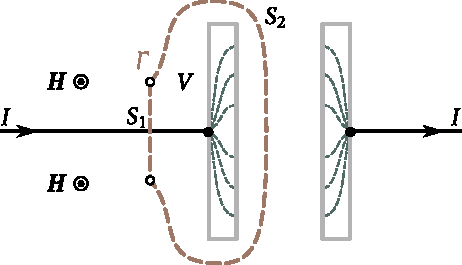
\includegraphics[scale=1]{figures/ch_09/fig_9_1.pdf}
		\caption[]{}
		\label{fig:9_1}
	\end{center}
	\vspace{-0.8cm}
\end{figure}

Let us take a circular loop $\Gamma$ enclosing the wire in which the current flows toward the capacitor and integrate \eqn{7_9} over surface $S_1$ intersecting the wire and enclosed by the loop:
\begin{equation*}
    \int_{S_1} \curlop{\vec{H}} \ccdot \derivec{S} = \int_{S_1} \vec{j} \ccdot \derivec{S}.
\end{equation*}

\noindent
Transforming the left-hand side according to Stokes's theorem we get the circulation of the vector $\vec{H}$ over loop $\Gamma$:
\begin{equation}\label{eq:9_6}
    \oint_{\Gamma} \vec{H} \ccdot \derivec{l} = \int_{S_1} \vec{j} \ccdot \derivec{S} = I
\end{equation}

\noindent
($I$ is the current charging the capacitor).
After performing similar calculations for surface $S_2$ that does not intersect the current-carrying wire (see \fig{9_1}), we arrive at the obviously incorrect relation
\begin{equation}\label{eq:9_7}
    \oint_{\Gamma} \vec{H} \ccdot \derivec{l} = \int_{S_2} \vec{j} \ccdot \derivec{S} = 0.
\end{equation}

\noindent
The result we have obtained indicates that for time-varying fields \eqn{7_9} stops being correct.
The conclusion suggests itself that this equation lacks an addend depending on the time derivatives of the fields.
For stationary fields, this addend vanishes.

That \eqn{7_9} is not correct for non-stationary fields is also indicated by the following reasoning.
Let us take the divergence of both sides of \eqn{7_9}:
\begin{equation*}
    \divop{(\curlop{\vec{H}})} = \divop{\vec{j}}.
\end{equation*}

\noindent
The divergence of a curl must equal zero [see \eqn{1_106}].
We, thus, arrive at the conclusion that the divergence of the vector $\vec{j}$ must also always equal zero.
But this conclusion contradicts the continuity equation \eqref{eq:5_11}.
Indeed, in non-stationary processes, $\rho$ may change with time (this, in particular, is what happens with the charge density on the plates of a capacitor being charged).
In this case in accordance with \eqn{5_11}, the divergence of $\vec{j}$ differs from zero.

To bring \eqns{5_11}{7_9} into agreement, Maxwell introduced an additional addend into the right-hand side of \eqn{7_9}.
It is quite natural that this addend should have the dimension of current density.
Maxwell called it the density of the displacement current.
Thus, according to Maxwell, \eqn{7_9} should have the
form
\begin{equation}\label{eq:9_8}
    \curlop{\vec{H}} = \vec{j} + \ab{\vec{j}}{d}.
\end{equation}

The sum of the conduction current and the displacement current is usually called the \textbf{total current}.
The density of the total current is
\begin{equation}\label{eq:9_9}
    \ab{\vec{j}}{tot} = \vec{j} + \ab{\vec{j}}{d}.
\end{equation}

If we assume that the divergence of the displacement current equals that of the conduction current taken with the opposite sign:
\begin{equation}\label{eq:9_10}
    \divop{\ab{\vec{j}}{d}} = - \divop{\vec{j}},
\end{equation}

\noindent
then the divergence of the right-hand side of \eqn{9_8}, like that of the left-hand side, will always be zero.

Substituting $\diffinpartial{\rho}{t}$ for $\divop{\vec{j}}$ in \eqn{9_10} in accordance with \eqn{5_11}, we get the following expression for the divergence of the displacement current:
\begin{equation}\label{eq:9_11}
    \divop{\ab{\vec{j}}{d}} = \diffinpartial{\rho}{t}.
\end{equation}

\noindent
To associate the displacement current with quantities characterizing the change in an electric field with time, let us use \eqn{2_23} according to which the divergence of the electric displacement vector equals the density of the extraneous charges:
\begin{equation*}
    \divop{\vec{D}} = 0.
\end{equation*}

\noindent
Time differentiation of this equation yields
\begin{equation*}
    \diffpartial{}{t} (\divop{\vec{D}}) = \diffpartial{\rho}{t}.
\end{equation*}

\noindent
Now, let us change the sequence of differentiation with respect to time and to the coordinates in the left-hand side.
As a result, we get the following. expression for the derivative of $\rho$ with respect to $t$:
\begin{equation*}
    \diffpartial{\rho}{t} = \divop{\parenthesis{ \diffpartial{\vec{D}}{t} }}.
\end{equation*}

\noindent
Introduction of this expression into \eqn{9_11} yields
\begin{equation*}
    \divop{\ab{\vec{j}}{d}} = \divop{\parenthesis{ \diffpartial{\vec{D}}{t} }}.
\end{equation*}

\noindent
Hence,
\begin{equation}\label{eq:9_12}
    \ab{\vec{j}}{d} = \diffpartial{\vec{D}}{t}.
\end{equation}

Using \eqn{9_12} in \eqn{9_8}, we arrive at the equation
\begin{equation}\label{eq:9_13}
    \curlop{\vec{H}} = \vec{j} + \diffpartial{\vec{D}}{t},
\end{equation}

\noindent
which, like \eqn{9_5}, is one of the fundamental equations in Maxwell's theory.

We must underline the fact that the term ``displacement current'' is purely conventional.
In essence, the displacement current is a time-varying electric field.
The only reason for calling the quantity given by \eqn{9_12} a ``current'' is that the dimension of this quantity coincides with that of current density.
Of all the physical properties belonging to a real current, a displacement current has only one---the
ability of producing a magnetic field.

The introduction of the displacement current determined by \eqn{9_12} has ``given equal rights'' to an electric field and a magnetic field.
It can be seen from the phenomenon of electromagnetic induction that a varying magnetic field sets up an electric field.
It follows from \eqn{9_13} that a varying electric field sets up a magnetic field.

There is a displacement current wherever there is a time-varying electric field.
In particular, it also exists inside conductors carrying an alternating electric current.
The displacement current inside conductors, however, is usually negligibly small in comparison with the conduction current.

We must note that \eqn{9_6} is approximate.
For it to become quite strict, we must add a term to its right-hand side that takes account of the displacement current due to the weak dispersed electric field in the vicinity of surface $S_1$.

Let us convince ourselves that the surface integral of the right-hand side of \eqn{9_8} has the same value for surfaces $S_1$ and $S_2$ (see \fig{9_1}).
Both the conduction current and the displacement current due to the electric field outside the capacitor ``flow'' through surface $S_1$.
Hence, for the first surface, we have
\begin{equation*}
    \text{Int}_1 = \int_{S_1} \vec{j} \ccdot \derivec{S} + \diff{}{t} \int_{S_1} \vec{D} \ccdot \derivec{S} = I + \diff{}{t} \ab{\Phi}{$1$,in}
\end{equation*}

\noindent
(we have changed the sequence of the operations of differentiation with respect to time and integration over the coordinates in the second addend).
The quantity designated by the letter $I$ is the current flowing in the conductor to the left-hand plate of the capacitor, $\ab{\Phi}{$1$,in}$ is the flux of the vector $\vec{D}$ flowing into the volume $V$ bounded by surfaces $S_1$ and $S_2$ (see \fig{9_1}).

For the second surface, $\vec{j}=0$, consequently
\begin{equation*}
    \text{Int}_2 = \diff{}{t} \int_{S_2} \vec{D} \ccdot \derivec{S} = \diff{}{t} \ab{\Phi}{$2$,out}
\end{equation*}

\noindent
where $\ab{\Phi}{$2$,out}$ is the flux of the vector $\vec{D}$ flowing out of volume $V$ through surface $S_2$.

The difference between the integrals is
\begin{equation*}
    \text{Int}_2 - \text{Int}_1 = \diff{}{t} \ab{\Phi}{$2$,out} - \diff{}{t} \ab{\Phi}{$1$,in} - I.
\end{equation*}

\noindent
The current $I$ can be represented as $\diffin{q}{t}$, where $q$ is the charge on a capacitor plate.
The flux passing inward through surface $S_1$ equals
the flux passing outward through the same surface taken with the opposite sign.
Substituting $-\ab{\Phi}{$1$,out}$ for $\ab{\Phi}{$1$,in}$ and $\diffin{q}{t}$ for $I$, we get
\begin{equation}\label{eq:9_14}
    \text{Int}_2 - \text{Int}_1 = \diff{}{t} \parenthesis{\ab{\Phi}{$2$,out} + \ab{\Phi}{$1$,out}} - \diff{q}{t} = \diff{}{t} \parenthesis{\Phi_D - q},
\end{equation}

\noindent
where $\Phi_D$ is the flux of the vector $\vec{D}$ through the closed surface formed by surfaces $S_1$ and $S_2$.
According to \eqn{2_25}, this flux must equal the charge enclosed by the surface.
In the given case, it is the charge $q$ on a capacitor plate.
Thus, the right-hand side of \eqn{9_14} equals zero.
It follows that the magnitude of the surface integral of the total current density vector does not depend on the choice of the surface over which the integral is being calculated.

We can construct current lines for the displacement current like those for the conduction current.
According to \eqn{2_35}, the electric displacement in the space between the capacitor plates equals the surface charge density on a plate: $D=\sigma$.
Hence,
\begin{equation*}
    \dot{D} = \dot{\sigma}.
\end{equation*}

\noindent
The left-hand side gives the density of the displacement current in the space between the plates, and the right-hand side-the density of the conduction current inside the plates.
The equality of these densities signifies that the lines of the conduction current uninterruptedly transform into lines of the displacement current at the boundary of the plates.
Consequently, the lines of the total current are closed.

\section{Maxwell's Equations}\label{sec:9_3}

The discovery of the displacement current permitted Maxwell to present a single general theory of electrical and magnetic phenomena.
This theory explained all the experimental facts known at that time and predicted a number of new phenomena whose existence was confirmed later on.
The main corollary of Maxwell's theory was the conclusion on the existence of electromagnetic waves propagating with the speed of light.
Theoretical investigation of the properties of these waves led Maxwell to the electromagnetic theory of light.

The theory is based on \textbf{Maxwell's equations}.
These equations play the same part in the science of electromagnetism as Newton's laws do in mechanics, or the fundamental laws in thermodynamics.

The \textbf{first pair of Maxwell's equations} is formed by \eqns{9_5}{7_3}:
\begin{align}
    \curlop{\vec{E}} &= - \diffpartial{\vec{B}}{t},\label{eq:9_5rev} \tag{9.5}\\
    \divop{\vec{B}} &= 0.\label{eq:7_3rev} \tag{7.3}
\end{align}

\noindent
The first of them relates the values of $\vec{E}$ to changes in the vector $\vec{B}$ in time and is in essence an expression of the law of electromagnetic
induction.
The second one points to the absence of sources of a magnetic field, \ie, magnetic charges.

The \textbf{second pair of Maxwell's equations} is formed by \eqns{9_13}{2_23}:
\begin{align*}
    \curlop{\vec{H}} &= \vec{j} + \diffpartial{\vec{D}}{t},\label{eq:9_13rev} \tag{9.13}\\
    \divop{\vec{D}} &= \rho.\label{eq:2_23rev} \tag{2.23}
\end{align*}

\noindent
The first of them establishes a relation between the conduction and displacement currents and the magnetic field they produce.
The second one shows that extraneous charges are the sources of the vector $\vec{D}$.

Equations \eqref{eq:9_5rev}, \eqref{eq:7_3rev}, \eqref{eq:9_13rev} and \eqref{eq:2_23rev} are Maxwell's equations in the differential form.
We must note that the first pair of equations includes only the basic characteristics of a field, namely, $\vec{E}$ and $\vec{B}$.
The second pair includes only the auxiliary quantities $\vec{D}$ and $\vec{H}$.

Each of the vector equations \eqref{eq:9_5rev} and \eqref{eq:9_13rev} is equivalent to three scalar equations relating the components of the vectors in the left-hand and right-hand sides of the equations.
Using Eqs. \eqref{eq:1_81} and \eqref{eq:1_92}-\eqref{eq:1_91}, let us present Maxwell's equation in the scalar form:
\begin{align}
    & \begin{cases}
        &\!\!\!\! \diffpartial{E_z}{y} - \diffpartial{E_y}{z} = - \diffpartial{B_x}{t}\\[8pt]
        &\!\!\!\! \diffpartial{E_x}{z} - \diffpartial{E_z}{x} = - \diffpartial{B_y}{t}\\[8pt]
        &\!\!\!\! \diffpartial{E_y}{x} - \diffpartial{E_x}{y} = - \diffpartial{B_z}{t}\\
    \end{cases}\label{eq:9_15}\\[5pt]
    & \quad\,\diffpartial{B_x}{x} + \diffpartial{B_y}{y} + \diffpartial{B_z}{z} = 0,\label{eq:9_16}
\end{align}

\noindent
(the first pair of equations),
\begin{align}
    & \begin{cases}
        &\!\!\!\! \diffpartial{H_z}{y} - \diffpartial{H_y}{z} = j_x + \diffpartial{D_x}{t}\\[8pt]
        &\!\!\!\! \diffpartial{H_x}{z} - \diffpartial{H_z}{x} = j_y + \diffpartial{D_y}{t}\\[8pt]
        &\!\!\!\! \diffpartial{H_y}{x} - \diffpartial{H_x}{y} = j_z + \diffpartial{D_z}{t}
    \end{cases}\label{eq:9_17}\\[5pt]
    & \quad\,\diffpartial{D_x}{x} + \diffpartial{D_y}{y} + \diffpartial{D_z}{z} = \rho,\label{eq:9_18}
\end{align}

\noindent
(the second pair of equations).

We get a total of $8$ equations including $12$ functions (three components each of the vectors $\vec{E}$, $\vec{B}$, $\vec{D}$, $\vec{H}$).
Since the number of equations is less than the number of unknown functions, \eqref{eq:9_5rev}, \eqref{eq:7_3rev}, \eqref{eq:9_13rev} and \eqref{eq:2_23rev} are not sufficient for finding the fields according to the given distribution of the charges and currents.
To calculate the fields, we must add equations relating $\vec{D}$ and $\vec{j}$ to $\vec{E}$ and also $\vec{H}$ to $\vec{B}$ to these equations.
They have the form
\begin{align}
    \vec{D} &= \varepsilon_0\varepsilon \vec{E}, \label{eq:2_21rev}\tag{2.21}\\
    \vec{B} &= \mu_0\mu \vec{H}, \label{eq:7_17rev}\tag{7.17}
    % \vec{j} &= \sigma \vec{E}. \label{eq:5_22rev}\tag{5:22}
\end{align}
\begin{equation}\label{eq:5_22rev}
    \vec{j} = \sigma \vec{E}. \tag{5.22}
\end{equation}

The collection of equations \eqref{eq:9_5rev}, \eqref{eq:7_3rev}, \eqref{eq:9_13rev} and \eqref{eq:2_23rev}, and \eqref{eq:2_21rev},
\eqref{eq:7_17rev}, \eqref{eq:5_22rev} forms the foundation of the electrodynamics of media at rest.

The equations
\begin{align}
    \oint_{\Gamma} \vec{E} \ccdot \derivec{l} &= - \diff{}{} \int_S \vec{B} \ccdot \derivec{S}, \label{eq:9_19}\\
    \oint_S \vec{B} \ccdot \derivec{S} &= 0, \label{eq:9_20}
\end{align}

\noindent
(the first pair) and
\begin{align}
    \oint_{\Gamma} \vec{H} \ccdot \derivec{l} &= \int_S \vec{j} \ccdot \derivec{S} + \diff{}{} \int_S \vec{B} \ccdot \derivec{S}, \label{eq:9_21}\\
    \oint_S \vec{D} \ccdot \derivec{S} &= \int_V \rho\, \deriv{V}, \label{eq:9_22}
\end{align}

\noindent
(the second pair) are \textbf{Maxwell's equations in the integral form}.

Equation \eqref{eq:9_19} is obtained by integration of \eqn{9_5} over arbitrary surface $S$ with the following transformation of the left-hand side according to Stokes's theorem into an integral over loop $\Gamma$ enclosing surface $S$.
Equation \eqref{eq:9_21} is obtained in the same way from \eqn{9_13}.
Equations \eqref{eq:9_20} and \eqref{eq:9_22} are obtained from \eqns{7_3}{2_23} by integration over the arbitrary volume $V$ with the following transformation of the left-hand side according to the Ostrogradsky-Gauss theorem into an integral over closed surface $S$ enclosing volume $V$.
